% FastLane poster, A1 landscape (841 x 594 mm), in the IIIT Hyderabad poster format (LTRC).
% Build (from poster/):  xelatex fastlane_poster.tex
% Figures:              .venv/bin/python poster/make_poster_figures.py   (from the repo root)
\documentclass{article}
\usepackage[paperwidth=841mm,paperheight=594mm,margin=0mm]{geometry}
\usepackage{fontspec}
\setmainfont{Helvetica Neue}
\usepackage{xcolor}
\usepackage{graphicx}
\usepackage{ragged2e}
\usepackage{tikz}
\usetikzlibrary{positioning,arrows.meta,calc}
\pagestyle{empty}
\setlength{\parindent}{0pt}
\setlength{\emergencystretch}{3em}
\setlength{\JustifyingParindent}{0pt}
\setlength{\RaggedRightParindent}{0pt}
\newcommand{\pval}[1]{\textit{p}\,=\,#1}

% Colours sampled from the template.
\definecolor{header}{HTML}{D4C7F4}
\definecolor{headline}{HTML}{0B0A08}
\definecolor{secpurple}{HTML}{45288A}
\definecolor{mint}{HTML}{E1EDEB}
\definecolor{mintc}{HTML}{E7F2F4}
\definecolor{beige}{HTML}{EFEAE4}
\definecolor{lightgrey}{HTML}{F2F2F2}
\definecolor{cstarborder}{HTML}{5D4275}
\definecolor{footerline}{HTML}{492D7A}
\definecolor{imgborder}{HTML}{8096A1}
\definecolor{ink}{HTML}{111111}
\definecolor{fl}{HTML}{EB6834}

% Type sizes for print at A1 (read from 1-2 m).
\newcommand{\bodysize}{\fontsize{26}{34}\selectfont}
\newcommand{\refsize}{\fontsize{19.5}{24.5}\selectfont}
\newcommand{\sechead}[1]{{\RaggedRight\fontsize{38}{44}\selectfont\bfseries\color{secpurple}#1\par}\vspace{5mm}}
\newcommand{\bul}[1]{\par\hangindent=1.1em\hangafter=1\makebox[1.1em][l]{\textbullet}#1\par\vspace{2.5mm}}
\newcommand{\refitem}[2]{\par\hangindent=1.6em\hangafter=1\makebox[1.6em][l]{[#1]}#2\par\vspace{1.5mm}}

% \panel{x}{y}{w}{h}{fill}: a background box, coordinates in mm from the top-left corner of the page.
\newcommand{\panel}[5]{\fill[#5] (#1mm,-#2mm) rectangle ++(#3mm,-#4mm);}
% \content{x}{y}{w}{text}: a text block with its top-left corner at (x, y).
\newcommand{\content}[4]{\node[anchor=north west, inner sep=0, text width=#3mm, align=justify, font=\bodysize, text=ink]
  at (#1mm,-#2mm) {#4};}
% \imagebox{x}{y}{w}{h}: white image area with the template's thin border.
\newcommand{\imagebox}[4]{\filldraw[fill=white, draw=imgborder, line width=0.6mm] (#1mm,-#2mm) rectangle ++(#3mm,-#4mm);}

\begin{document}
\begin{tikzpicture}[remember picture, overlay, shift={(current page.north west)}]

% ---------------------------------------------------------------- header
\panel{0}{0}{841}{68}{header}
\begin{scope}
  \clip (0,0) rectangle (841mm,-68mm);
  \foreach \i in {0,...,9} {
    \draw[white, opacity=0.55, line width=0.5mm]
      ($(420mm,-75mm)+(\i*7mm,0)$) .. controls ($(470mm,-20mm)+(\i*6mm,0)$) and ($(560mm,10mm)+(\i*5mm,0)$) .. ($(700mm,5mm)+(\i*4mm,0)$);
  }
\end{scope}
\node[anchor=north west, inner sep=0, text width=720mm, align=left, font=\fontsize{64}{74}\selectfont\bfseries, text=headline]
  at (15mm,-10mm) {FastLane: A Voice Agent That Routes Each Turn\\Between a Small and a Large Model};
\node[anchor=north east, inner sep=0] at (829mm,-14mm) {
\includegraphics[width=72mm]{iiith_logo.png}};

% ---------------------------------------------------------------- column 1
\panel{12}{80}{236}{191}{mint}
\content{21}{89}{218}{\sechead{ABSTRACT}
Most voice agents send every turn to a large API model, which is slow and costly, although most turns of a booking
call are easy~[1,\,2]. FastLane books, changes and cancels movie tickets, bus tickets and restaurant tables for
Indian-English callers. A fine-tuned Qwen2.5-3B~[3] answers every turn first and passes only hard turns to
gpt-oss-120b~[4] or to staff, while a gateway enforces the booking rules and a read-back confirmation in code. On 120
simulated calls FastLane succeeds in 90\% (large model alone: 82\%) with 78\% fewer large-model calls and no
booking change the caller did not confirm. It is not faster on our hardware.}

\panel{12}{278}{236}{281}{mint}
\content{21}{287}{218}{\sechead{METHODOLOGY}\RaggedRight
\bul{\textbf{Practice world:} SQLite booking system for three domains, 11 tools, 360 scripted test calls.}
\bul{\textbf{Safety in code:} rules, read-back before every change and identity checks live in a gateway, not in the prompt.}
\bul{\textbf{Training data without an LLM teacher:} rule-based callers and an oracle agent run 650 practice calls through the real agent; QLoRA~[5] on a Kaggle T4, served as 4-bit MLX on a laptop.}
\bul{\textbf{Evaluation:} 12 systems, a simulated caller (Qwen2.5-7B) as in $\tau$-bench~[6], paired McNemar tests, and every failed call read by hand.}}

\imagebox{21}{466}{218}{85}
\begin{scope}[shift={(21mm,-466mm)}, font=\fontsize{17}{20}\selectfont,
  box/.style={draw=secpurple!70, line width=0.5mm, rounded corners=1.5mm, align=center, fill=white, inner sep=1.5mm},
  arr/.style={-{Stealth[length=3.2mm]}, line width=0.6mm, color=ink}]
  \node[box, minimum width=27mm, minimum height=18mm] (caller) at (17mm,-20mm) {Caller\\speaks};
  \node[box, minimum width=34mm, minimum height=18mm] (stt) at (60mm,-20mm) {Speech to\\text [7,\,8]};
  \node[box, minimum width=48mm, minimum height=18mm, fill=fl!15, draw=fl] (small) at (120mm,-20mm) {\textbf{Small model}\\Qwen2.5-3B + LoRA};
  \node[box, minimum width=44mm, minimum height=18mm, fill=secpurple!10] (large) at (188mm,-20mm) {\textbf{Large model}\\gpt-oss-120b};
  \node[box, minimum width=34mm, minimum height=18mm] (staff) at (24mm,-64mm) {Staff\\hand-off};
  \node[box, minimum width=86mm, minimum height=18mm] (gw) at (101mm,-64mm) {\textbf{Gateway:} tools, rules,\\read-back, identity check};
  \node[box, minimum width=44mm, minimum height=18mm] (tts) at (188mm,-64mm) {Spoken\\reply};
  \draw[arr] (caller) -- (stt);
  \draw[arr] (stt) -- (small);
  \draw[arr] (small) -- node[above, font=\fontsize{15}{17}\selectfont]{hard} (large);
  \draw[arr] (small.south) -- node[right, font=\fontsize{15}{17}\selectfont]{easy} (small.south |- gw.north);
  \draw[arr] (large.south west) -- (gw.north east);
  \draw[arr] (small.south west) -- node[above left, font=\fontsize{15}{17}\selectfont, inner sep=0.5mm]{red flag} (staff.north east);
  \draw[arr] (gw) -- (tts);
\end{scope}

% ---------------------------------------------------------------- column 2
\panel{254}{80}{382}{225}{beige}
\content{263}{89}{364}{\sechead{RESULTS}
Same 48 test calls for every system (FastLane and B1 also on 120), one seed, gpt-oss-120b on Groq. With rules in
code FastLane made \textbf{no unconfirmed booking change}, against 44 of 120 calls for B1 (large model only) and 31 of
48 for A3 (rules only in the prompt). It succeeded at least as often as B1 (90.0\% vs.\ 81.7\%, \pval{0.087}) with
78\% fewer large-model calls, but B1 is faster (p95 3.0\,s vs.\ 6.8\,s per turn).}
\imagebox{263}{168}{364}{131}
\node[anchor=center, inner sep=0] at (445mm,-233.5mm) {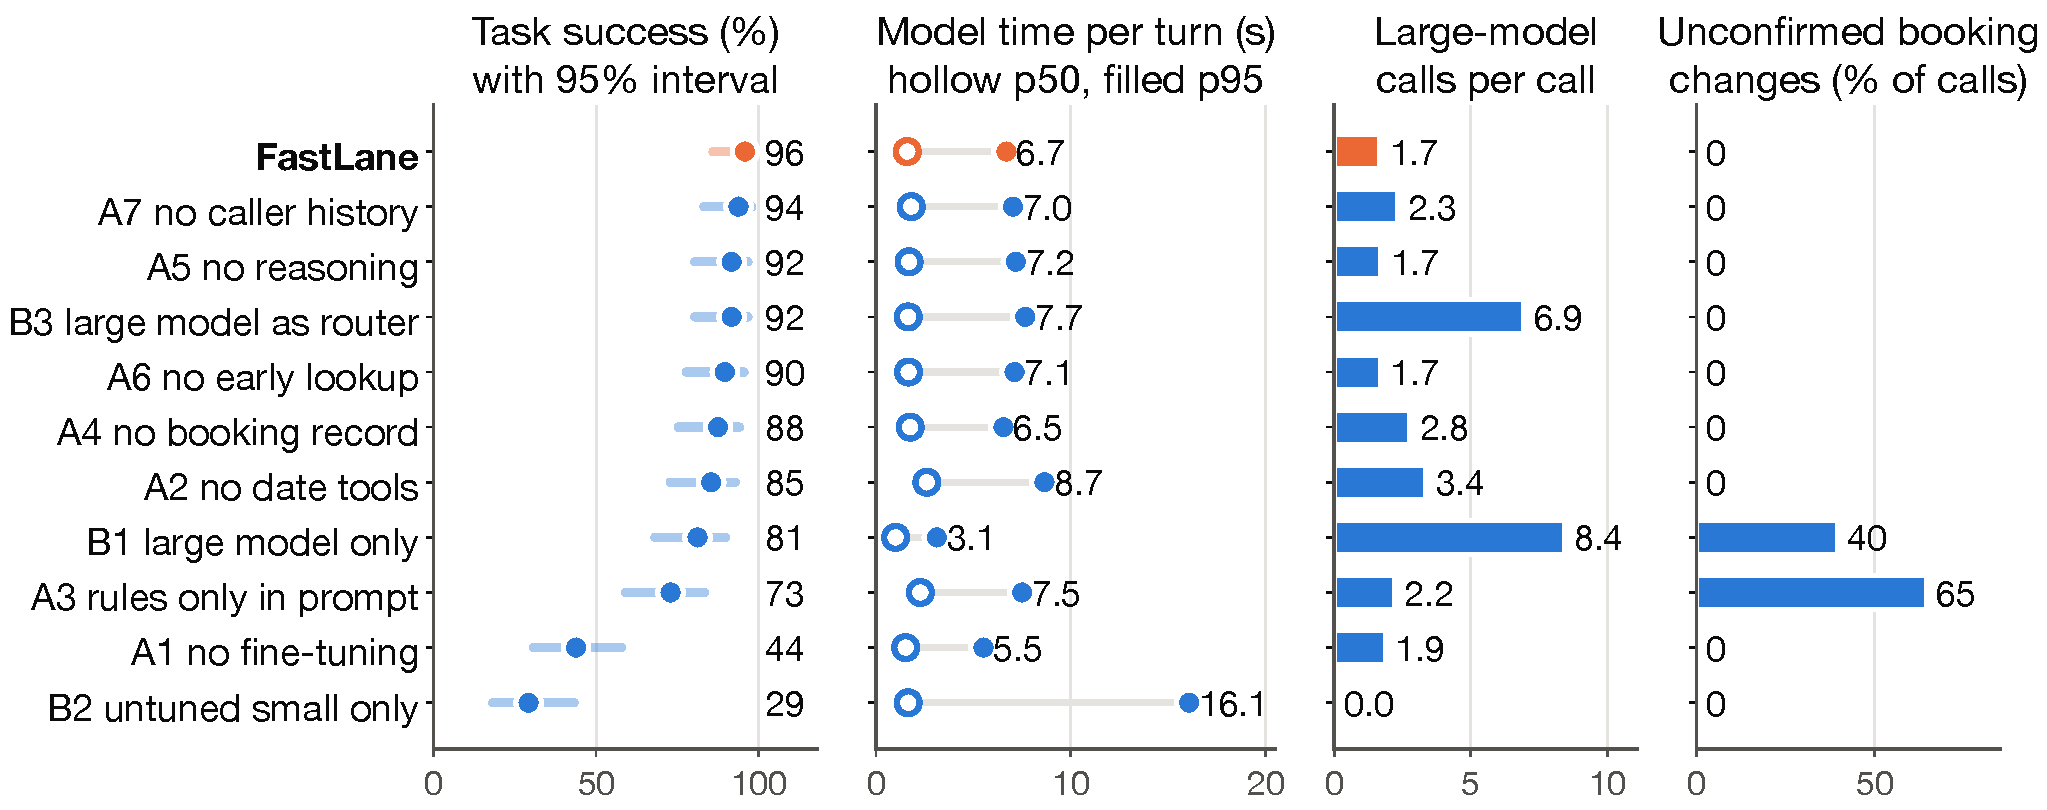
\includegraphics[width=350mm,height=125mm,keepaspectratio]{figures/results_poster.pdf}};

\panel{254}{311}{188}{248}{lightgrey}
\content{263}{320}{170}{\sechead{FINE-TUNING MATTERS}
On 267 held-out steps the untuned 3B model fills tool arguments exactly in 27\% of steps, the tuned one in 99\%.
End to end, the untuned model succeeds in 29\% of calls alone (B2) and in 44\% inside FastLane (A1), against
96\%. A model never trained on restaurants still gets 37 of 40 restaurant calls right.}
\imagebox{263}{458}{170}{93}
\node[anchor=center, inner sep=0] at (348mm,-504.5mm) {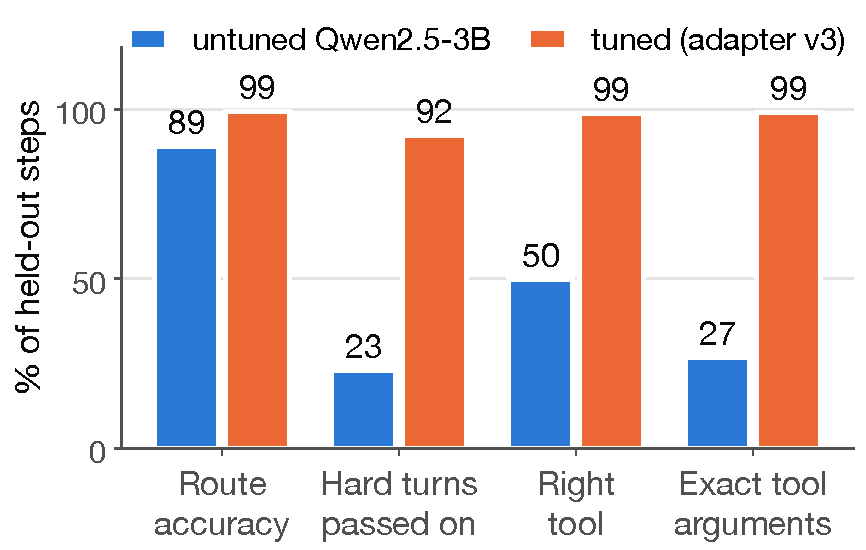
\includegraphics[width=162mm,height=87mm,keepaspectratio]{figures/finetune_poster.pdf}};

\panel{448}{311}{188}{248}{lightgrey}
\content{457}{320}{170}{\sechead{READING EVERY FAILURE}
Half of FastLane's 12 failures came from the simulated caller, mostly by not changing its mind as scripted. The
5 agent errors (a guessed bus origin, a false ``cancelled'', a contradicted policy text) led to four checks in
code. They removed those errors, but success in a rerun moved only within noise (13 of 120 calls changed,
\pval{0.58}).}
\imagebox{457}{458}{170}{93}
\node[anchor=center, inner sep=0] at (542mm,-504.5mm) {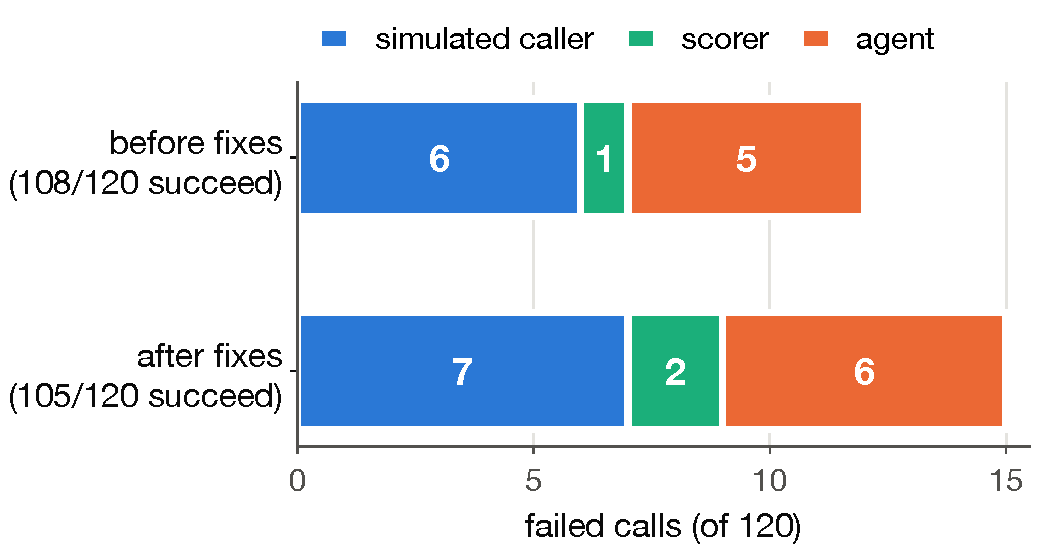
\includegraphics[width=162mm,height=85mm,keepaspectratio]{figures/failures_poster.pdf}};

% ---------------------------------------------------------------- column 3
\filldraw[fill=white, draw=cstarborder, line width=0.9mm] (642mm,-79mm) rectangle ++(188mm,-55mm);
\node[anchor=center, inner sep=0, font=\fontsize{80}{80}\selectfont, text=black] at (736mm,-99mm) {LTRC};
\node[anchor=center, inner sep=0, font=\fontsize{23}{27}\selectfont, text=black] at (736mm,-123mm) {Language Technologies Research Centre};

\panel{642}{140}{188}{420}{mintc}
\content{651}{149}{170}{\sechead{CONCLUSION AND\\FUTURE WORKS}\RaggedRight
\bul{A tuned 3B model handles four of five turns, with 78\% fewer large-model calls.}
\bul{Safety belongs in code: no unconfirmed changes, vs.\ 37--65\% of calls with rules in the prompt.}
\bul{No speed gain here: a hosted 120B model beats a 3B model on a laptop.}
\bul{Next: a faster small-model path, retraining on corrected data, real callers.}
\vspace{6mm}
\sechead{ACKNOWLEDGMENT}
\justifying We thank the instructors and teaching assistants of the LMA 2026 course for their guidance and feedback.
\par\vspace{7mm}
\sechead{REFERENCES}
\refsize\RaggedRight
\refitem{1}{L.~Chen, M.~Zaharia, J.~Zou. FrugalGPT. TMLR 2024.}
\refitem{2}{I.~Ong et al. RouteLLM. ICLR 2025.}
\refitem{3}{Qwen Team. Qwen2.5 technical report, 2024.}
\refitem{4}{OpenAI. gpt-oss-120b \& gpt-oss-20b model card, 2025.}
\refitem{5}{T.~Dettmers et al. QLoRA. NeurIPS 2023.}
\refitem{6}{S.~Yao et al. $\tau$-bench. ICLR 2025.}
\refitem{7}{A.~Radford et al. Whisper. ICML 2023.}
\refitem{8}{T.~Javed et al. Svarah. Interspeech 2023.}
\vspace{3mm}
{\bfseries Code:} github.com/Sankalp0109/\\FastLane-Adaptive-Voice-Agent}

% ---------------------------------------------------------------- footer
\draw[footerline, line width=1.1mm] (14mm,-565mm) -- (826mm,-565mm);
\node[anchor=west, inner sep=0, font=\fontsize{24}{28}\selectfont\itshape, text=black] at (21mm,-573mm)
  {Author names: Noel Alex Jacob, Aviral Tyagi, Sankalp Chaturvedi, KSPSVLN Siddardha Kumar Kavuri};
\node[anchor=west, inner sep=0, font=\fontsize{24}{28}\selectfont\itshape, text=black] at (21mm,-584mm)
  {Email IDs: noel.jacob@students.iiit.ac.in, aviral.tyagi@students.iiit.ac.in,
   sankalp.chaturvedi@students.iiit.ac.in, kspsvlnsiddardha.k@students.iiit.ac.in};

\end{tikzpicture}
\end{document}
